\documentclass[11pt]{article}
\usepackage[preprint]{acl}
\usepackage{times}
\usepackage{latexsym}
\usepackage[T1]{fontenc}
\usepackage[utf8]{inputenc}
\usepackage{microtype}
\usepackage{graphicx}
\usepackage{booktabs}
\usepackage{array}
\usepackage{float}
\usepackage{amsmath}
\usepackage{listings}
\usepackage{tikz}
\usetikzlibrary{arrows.meta,positioning}
\newcommand{\bc}{BrainCode}
\newcommand{\code}[1]{\texttt{#1}}
\lstset{basicstyle=\ttfamily\footnotesize,columns=fullflexible,keepspaces=true,
 breaklines=true,showstringspaces=false,frame=single,framerule=.3pt,
 rulecolor=\color{gray},xleftmargin=3pt,xrightmargin=3pt,aboveskip=6pt,belowskip=4pt}
\title{BrainCode: Agent-Created Language for\ Natural-Language Tasks and Conversations}
\author{Lia Soffer \quad Noam Yehezkel \\
 Tel Aviv University}
\date{}
\begin{document}
\maketitle
\begin{abstract}
Formal intermediate languages could expose how large language models interpret natural language. We ask whether agents can construct such a language, whether models interpret it consistently, and whether translation improves reasoning. We introduce \bc{}, a typed language for tasks and conversations, intended for model comparison, reasoning decomposition, and prompt formalization or compression. A multi-model syntax loop and retrieval-assisted glossary swarm pursue coverage, determinism, expressivity, reasoning improvement, and human interpretability. Development across six datasets produces 657 active glossary records. On 18 shared held-out items with three repeats, coverage ranges from 44.4\% for Claude Sonnet to 92.6\% for Claude Haiku among four main conditions; additional OpenAI trials largely fail acceptance. Symbol preferences and strictness differ across models, and round-trip reconstruction loses detail. On 50 BBEH-mini items, Llama 3.1 8B accuracy falls from 12.0\% to 0.7\% after in-context translation. \bc{} exposes behavioral differences, but does not yet establish a model-neutral representation or a reasoning benefit.
\end{abstract}

\section{Introduction}
Natural language permits multiple interpretations of tasks, beliefs, and changing intentions. An intermediate representation could name objects, distinguish proposed actions from observed events, and preserve who asserted which claim. We investigate whether language-model agents can build such a representation and whether it transfers beyond its creators.

\paragraph{Related work.}
Abstract Meaning Representation separates sentence meaning from surface form through a graph representation \citep{banarescu2013amr}. \bc{} shares the aim of explicit semantic structure, but also represents action plans, conversational turns, replies, and revisions, with a vocabulary expanded by agents. This broader scope increases the difficulty of defining a stable interpretation.
Structured intermediate steps can help language-model reasoning when paired with suitable mechanisms. \citet{yao2023react} interleave reasoning and environmental actions; \citet{gao2023pal} delegate computations to a program interpreter; and \citet{zelikman2023parsel} compose natural-language decompositions into programs. These findings motivate our reasoning hypothesis, but their benefits cannot be assumed to transfer to a newly invented notation without execution or training. Automatic textbook formalization further illustrates the value of machine-checkable targets \citep{gloeckle2026formalization}; our checker verifies selected language constraints, not proofs or semantic equivalence. Prompt compression offers another motivation: \citet{jiang2023llmlingua} compress prompts while assessing downstream performance. We consider formalization and compression potential uses of \bc{}, without claiming token savings.

\paragraph{Our work and objectives.}
We construct a language between a programming language and natural language: explicit typed structure constrains composition, while many primitive meanings remain documented in prose. Possible uses are comparative research on model interpretations and linguistic tendencies, reasoning-task decomposition, and prompt formalization or compression. We operationalize five objectives. \emph{Coverage} is the fraction of attempted translations accepted under a frozen specification and glossary, including errors in the denominator. \emph{Determinism} is stability of symbol-use distributions across repeated translations and models; lower divergence is better. \emph{Expressivity} is preservation of source information through encoding and decoding, approximated by reconstruction similarity. \emph{Improvement} is the accuracy difference between solving from a translated representation and solving from the original input. \emph{Human interpretability} means that a reader can identify the roles, references, and intended meaning of statements from the specification and glossary. We maintain the last objective through readable names, examples, and human review; we do not quantitatively evaluate it or claim validated usability.

\paragraph{Research questions.}
\textbf{RQ1:} How stable or model-dependent is translation, and can its variation support comparative analysis of model behavior? We examine determinism alongside coverage. \textbf{RQ2:} Can agents construct a usable language for heterogeneous natural-language material? We examine coverage, expressivity, and the interpretability-oriented design process. \textbf{RQ3:} Can an intermediate language improve reasoning through explicit decomposition? We compare direct and \bc{}-mediated solving. These exploratory questions concern one artifact; generating syntax need not establish semantic understanding.

\section{BrainCode}
\label{sec:braincode}
\subsection{Syntax creation}
The syntax loop assigns a Searcher to propose constructs, a Shaper to revise the specification, a Critic to test examples, and a Documenter to maintain definitions and glossary entries. The configuration uses Gemini 3.1 Pro Preview as Searcher, GPT-5.6 Terra as Critic, and Claude Sonnet 5 as Documenter; the Shaper rotates among them, with configured fallbacks. Starting from flat Python-like statements, explicit attribute/content distinctions, and conversation turns, prompts emphasize faithful representation, minimal primitives, explicit typing, bounded control flow, and readable names.

Proposals undergo simulated translations, critique, and documentation checks, with up to three reworks. Human hard constraints can block acceptance; other unresolved issues may be deferred. Acceptance is qualitative. The resulting syntax uses typed tasks, actions distinct from checks, immutable bindings, bounded iteration, and explicit reply and revision links.

We subsequently compared and merged the syntax-loop product with Guy's supplied design template, adding the separation between descriptive \code{TERM}s, attributed \code{CLAIM}s, reasoning \code{LINK}s, and observed-event \code{RECORD}s while retaining the task and conversation structure. These distinctions support provenance and reduce confusion between describing and executing an action, at the cost of more categories and a larger interpretation burden. The migration therefore improves representational explicitness without establishing that models apply the distinctions consistently.

\subsection{Glossary creation with a swarm}
The adapted swarm infrastructure runs bounded batches of containerized translators, then migration and inspection stages (Figure~\ref{fig:pipeline}). Humans still repaired runtime problems and made a small number of language corrections, so the final language reflects both agent proposals and human decisions.

\begin{figure}[t]
\centering
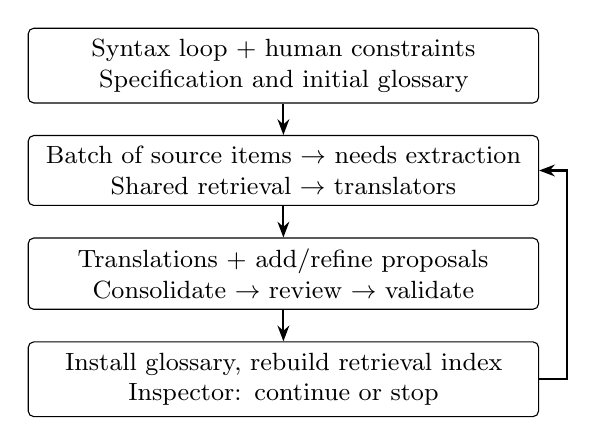
\begin{tikzpicture}[node distance=4mm, every node/.style={font=\small,align=center},
 box/.style={draw,rounded corners=2pt,text width=6.2cm,inner sep=4pt},
 arr/.style={-{Stealth[length=2mm]},thick}]
\node[box] (a) {Syntax loop + human constraints\\Specification and initial glossary};
\node[box,below=of a] (b) {Batch of source items $\rightarrow$ needs extraction\\Shared retrieval $\rightarrow$ translators};
\node[box,below=of b] (c) {Translations + add/refine proposals\\Consolidate $\rightarrow$ review $\rightarrow$ validate};
\node[box,below=of c] (d) {Install glossary, rebuild retrieval index\\Inspector: continue or stop};
\draw[arr] (a)--(b);\draw[arr] (b)--(c);\draw[arr] (c)--(d);
\draw[arr] (d.east)--++(.35,0)|-(b.east);
\end{tikzpicture}
\caption{Language construction. The glossary changes between development batches. Evaluation freezes both the specification and the glossary.}
\label{fig:pipeline}
\end{figure}

\paragraph{Data and loop.}
We assemble 42,180 local records from six datasets. Three contain relatively constrained tasks or action trajectories: Mind2Web for web interaction \citep{deng2023mind2web}, ALFRED for household instructions \citep{shridhar2020alfred}, and the full SWE-bench collection for software issues \citep{jimenez2024swebench}. Three provide more open-ended interactions: PRISM \citep{kirk2024prism}, PATHs writing conversations \citep{mysore2025paths}, and ThoughtTrace \citep{jin2026thoughttrace}. This closed/open grouping does not imply a unique correct output for every task. Local 80/20 splits use seed 42, with ALFRED grouped by trial to avoid splitting descriptions of the same trial. These local splits test new items within known sources, not official benchmark splits or unseen domains.

The planned development pool contains 500 training items per dataset, processed in batches of 30. Translators attempt faithful encodings and propose missing entries or refinements. Pre-migrators merge overlapping suggestions, a consolidator reconciles them, drafters prepare entries, and a stronger review stage can approve, replace, drop, or add proposals. Host-side validation precedes installation and retrieval reindexing. The inspector stops when accepted additions are at most two and refinements at most five, at least 80\% of translators finish, and migration is installed or validly skipped.

\begin{figure*}[t]
\centering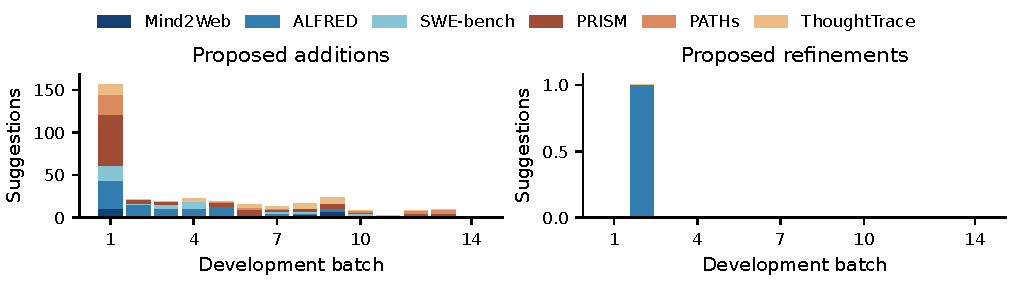
\includegraphics[width=\textwidth]{suggestions.pdf}
\caption{Proposed glossary additions and refinements in 14 development batches of 30 items. Blue shades identify the three relatively closed-ended task datasets; warm shades identify open-ended dialogue datasets. Counts are proposals, not necessarily accepted entries. The changing glossary and batches preclude interpreting this as a held-out learning curve.}
\label{fig:suggestions}
\end{figure*}

Only 420 items in 14 batches were processed before stopping, rather than the planned 3,000. There were 322 successful development translations, with batch success rising from 5/30 to 30/30, non-monotonically. Figure~\ref{fig:suggestions} shows the initial burst of vocabulary requests and later residual gaps. Historical growth from 329 records reached 685 before consolidation; the final frozen representation has 657 active records. Development success is not directly comparable with final held-out coverage because the language, examples, and checking rules evolved.

\paragraph{Retrieval and checking.}
A needs extractor identifies source-linked actions, objects, negation, temporal relations, and speech or claim requirements, with a heuristic fallback. Segments of roughly 400 characters retain source references linking retrieval to the original need. Retrieval combines exact aliases with light stemming, BM25 lexical ranking, and multilingual MiniLM embeddings. It gathers 15 candidates per channel, combines rankings with reciprocal-rank fusion ($k=60$), and reranks using 0.55 fusion score plus 0.45 context similarity and a small kind bonus. It retains 12 non-exact candidates plus exact matches, expands dependencies up to three levels and related entries by one hop, and includes shared rules. A widening operation increases candidates to 40 per channel and retains 30. Context used for reranking is capped at 600 characters.

Translators can retrieve, search, inspect entries, widen retrieval, and check outputs; migration rebuilds the in-memory index and embedding cache. The checker detects symbol occurrences, missing or unknown heads, invalid group atoms, retired entries, and opaque fallbacks; it is not a complete semantic validator. In successful outputs, long natural-language quotations of eight or more words are restricted except for designated exact-wording roles such as names and titles. This discourages passing untranslated prose through the formal layer, but can itself affect acceptance.

\subsection{Language and glossary}
\bc{} distinguishes \code{MODE REQUEST}, which specifies intended work, from \code{MODE TRACE}, which records a conversation or trajectory. An \code{ENTRYPOINT} names a \code{TASK} or \code{CONVO}. Typed terms describe entities and activities; actions request effects, checks test conditions, and claims carry attribution or epistemic status. Named immutable bindings expose dependencies instead of hiding nested calls. Conditionals and bounded iteration structure tasks. Conversation turns identify speakers, support \code{REPLY\_TO}, and distinguish whole-turn revisions from amendments to particular claims.

The glossary defines signatures and meanings (Table~\ref{tab:glossary}). Eight lexical groups avoid enumerating every possible value. Six permit normalized labels for objects, genres, foods, animals, colors, and platforms; two use country and currency standards. An atom such as \code{object\_label::mug} preserves an object's lexical identity, but does not supply an executable world model or a fully formal definition of a mug. This boundary between open labels and defined semantics becomes important in failures.

\begin{table}[t]
\centering\small
\begin{tabular}{lr@{\qquad}lr}
\toprule
Kind & Count & Kind & Count\\\midrule
Value &315& Constructor&84\\
Claim relation&63&Structural&52\\
Operation&38&Composite&27\\
Category rule&27&Rule&14\\
Speech act&11&Attribute&8\\
Lexical group&8&Link&5\\
Example&5&\textbf{Active total}&\textbf{657}\\
\bottomrule
\end{tabular}
\caption{Active records in glossary version g19. Two deprecated composite records are excluded from the 659 stored records. Entries include rules and examples as well as symbols.}
\label{tab:glossary}
\end{table}

\paragraph{Translation examples.}
The task below represents ``Move two pillows from the sofa onto the armchair,'' adapted from the shipped examples with shorter local binding names. The action produces references reused by the loop.
\begin{lstlisting}
MODE REQUEST
ENTRYPOINT MovePillows
TASK MovePillows {
 ACTION pick_up(
  target=object_label::pillow, quantity=2,
  source=object_label::sofa)
  -> pillows : LIST[REF[STRING]]
 FOR EACH item IN pillows {
  ACTION place(target=item,
   destination=object_label::armchair,
   relation=on)
 }
}
\end{lstlisting}
The following short, constructed conversation illustrates a shared term and reply: user, ``Shall we rinse the mug?''; agent, ``I suggest rinsing it.'' It demonstrates the notation rather than adding an evaluated success.
\begin{lstlisting}
MODE TRACE
ENTRYPOINT Conversation
CONVO Conversation {
 TURN t1 SPEAKER=USER {
  TERM activity(verb="rinse",
   object=object_label::mug) -> a : TERM
  UTTER ask(target=a)
 }
 TURN t2 SPEAKER=AGENT REPLY_TO t1 {
  UTTER propose(target=t1.a)
 }
}
\end{lstlisting}
The activity is described, not executed. Both examples remain partly dependent on a reader's interpretation of documented primitives.

\section{Evaluations}
\label{sec:eval}
\subsection{Design and coverage (RQ1--RQ2)}
Evaluation freezes the language at version 19.0.0-draft.2-lexical-groups and glossary g19. We sample eight local test items per dataset (48 total), capped at 6,000 characters, using seed 2026. Three items per dataset form a shared 18-item subset. Each model condition attempts three translations per item. All conditions share the translator toolkit and precomputed item needs and retrieval, controlling initial evidence but not subsequent tool use or rule interpretation.

Both Gemini conditions complete 144 attempts each; Claude Sonnet, Claude Haiku, and o4-mini complete 54 each, totaling 450 attempts. The Gemini comparison changes effort on the same Flash model, rather than comparing two model sizes. Model names in Table~\ref{tab:coverage} are the recorded experiment labels; Appendix~\ref{sec:repro} specifies endpoint identifiers. Two additional GPT conditions were interrupted and are reported separately. We retain infrastructure errors in coverage denominators and distinguish explicit translation failure from errors or rejected successes.

\begin{table}[t]
\centering\small
\begin{tabular}{lrrrr}
\toprule
Condition & S/F/E & Cov.\% & Miss. & All\%\\\midrule
Flash high &49/2/3&90.7&1.0&91.0\\
Flash &46/4/4&85.2&1.8&88.9\\
Sonnet 5.5 &24/30/0&44.4&1.8&---\\
Haiku 4.5 &50/4/0&92.6&2.5&---\\
o4-mini &4/46/4&7.4&2.4&---\\\midrule
GPT-6.1 Sol$^*$ &0/19/4&0.0&---&---\\
GPT-6 Luna$^*$ &0/19/3&0.0&---&---\\
\bottomrule
\end{tabular}
\caption{Shared-set coverage: successes/failures/errors (S/F/E) out of 54 attempts; Miss. is mean reported missing symbols per failed attempt. All is coverage over 144 Gemini attempts. $^*$Incomplete diagnostic samples of 23 and 22 attempts, respectively, not balanced comparisons.}
\label{tab:coverage}
\end{table}

\begin{figure*}[t]
\centering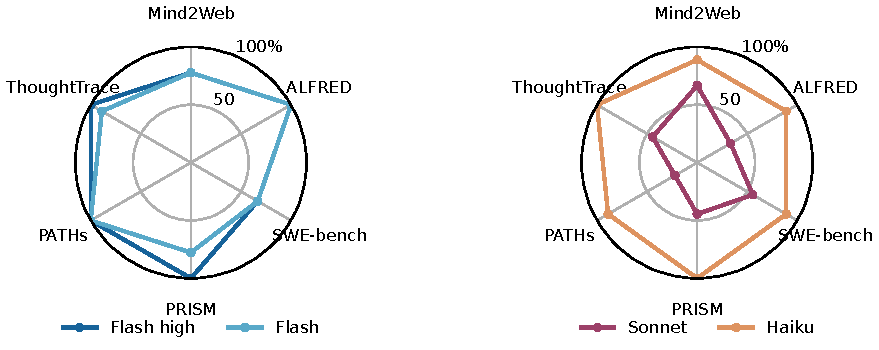
\includegraphics[width=.88\textwidth]{coverage-radar.pdf}
\caption{Shared-set coverage by dataset: nine attempts (three items, three repeats) per model and axis. The two panels have identical scales. Variation reflects both item difficulty and model-specific interpretation; each axis is based on only three distinct items.}
\label{fig:radar}
\end{figure*}

Haiku has the highest shared coverage, followed by high-effort Flash, Flash, and Sonnet. Therefore the data do not support a blanket advantage of Gemini over Claude, nor a monotonic relationship with nominal model strength. The per-dataset profiles in Figure~\ref{fig:radar} show additional variation: Sonnet accepts relatively more web tasks than PATHs conversations, while Haiku maintains high coverage across sources.

\paragraph{Why OpenAI trials failed.}
The stored GPT-6.1 Sol and GPT-6 Luna trials contain no accepted successes. Qualitative inspection suggests strict semantic readings: they request dedicated constructors such as \code{flight\_search\_request}, \code{job\_search}, or \code{search\_request} instead of using general \code{activity}, \code{requirement}, or \code{search\_web} constructs. Their objections concern describing a requested task versus executing it or assigning an unspecified meaning. The saved snapshot contains 71 constructor additions among 129 proposals. Some outputs are otherwise coherent, including Luna translations structurally similar to accepted Sonnet outputs; real shared gaps, such as \code{unit\_watt}, also remain. Zero acceptance therefore need not imply inability to write the notation.

We tried o4-mini as an additional comparison, but only 4/54 attempts succeeded. Inspection also found natural-language quotation and other attempts to bypass representational restrictions, which were disallowed where they violated the gate. We exclude OpenAI conditions from the main determinism and expressivity comparisons; we retain o4-mini's symbol profile and appendix plots solely as failure-confounded diagnostics. The model differences suggest compatibility with the Gemini-led glossary process, but lenient versus strict interpretation is an alternative to model-specific overfitting.

\subsection{Determinism (RQ1)}
For each translation, we count recognized glossary-symbol occurrences and lexical-group atoms, excluding quoted literals, comments, and structural/rule/example tokens. We normalize counts into distributions. For distributions $P,Q$ over their union of symbols, with $M=(P+Q)/2$, we use base-2 Jensen--Shannon divergence:
\begin{equation}
\operatorname{JS}(P,Q)=\tfrac12 D_{\mathrm{KL}}(P\|M)+\tfrac12 D_{\mathrm{KL}}(Q\|M).
\end{equation}
It lies in $[0,1]$; zero means identical frequency distributions, not identical programs or meanings. Between-model JS compares counts pooled over the shared sample. Self-divergence averages all repeat-pair divergences within each item, then averages items with at least two usable runs. We use the implemented arithmetic means; an earlier design proposed harmonic averaging. Accepted and explicitly failed translations contribute; errors do not. Partial outputs can therefore affect both measures.

\begin{figure*}[t]
\centering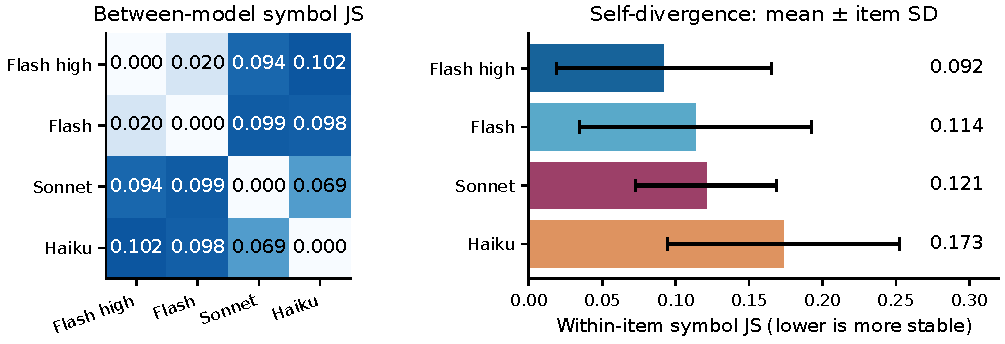
\includegraphics[width=\textwidth]{determinism.pdf}
\caption{Determinism on the shared sample. Left: JS between pooled symbol distributions. Right: mean within-item repeat divergence, with standard deviation across items (not confidence intervals). Flash conditions have 17 eligible items each; Sonnet and Haiku have 18. Lower values indicate more similar symbol usage.}
\label{fig:determinism}
\end{figure*}

Figure~\ref{fig:determinism} shows much closer pooled symbol use between Flash conditions (0.020) than across Gemini and Claude (0.094--0.102); Sonnet--Haiku divergence is 0.069. Mean self-divergence is 0.092 for high-effort Flash, 0.114 for Flash, 0.121 for Sonnet, and 0.173 for Haiku. High coverage and repeat stability thus need not coincide: Haiku covers more inputs but varies more between runs. Neither pooled similarity nor self-stability demonstrates fidelity to the source.

\begin{figure*}[t]
\centering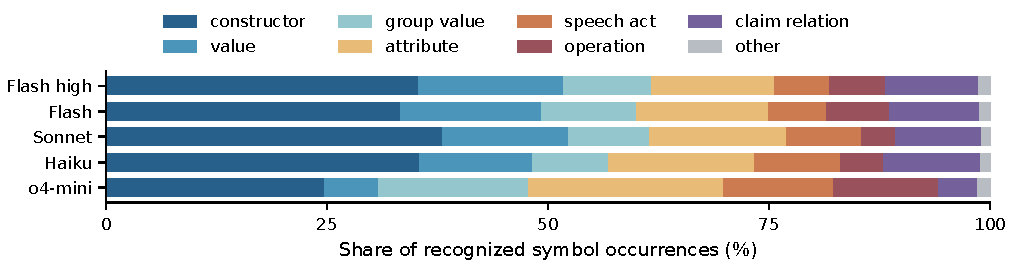
\includegraphics[width=.96\textwidth]{type-mix.pdf}
\caption{Normalized type mix of recognized symbol occurrences on the shared set, including explicit failures. Four main conditions have similar broad profiles despite different coverage. o4-mini is shown diagnostically; its 7.4\% coverage makes a direct comparison of successful language use inappropriate. ``Other'' combines links and composites; group values are lexical-group atoms.}
\label{fig:types}
\end{figure*}

Broad type distributions are closer than individual symbol distributions: main-condition pairwise type JS ranges from 0.0007 to 0.0071. Figure~\ref{fig:types} gives no simple ordering of type preferences by success rate. o4-mini differs more (type JS 0.050--0.062 versus the other conditions), but its partial failures confound interpretation. The saved Claude-generated qualitative report describes more action/task-oriented encodings in Gemini and more explicit utterance-oriented encodings in Claude, with Sonnet often constructing more terms and Haiku varying its decomposition. Selected high-divergence cases explain patterns rather than estimate their prevalence. Together with the coverage radar, they reveal representational preferences, without validating a taxonomy of linguistic abilities.

\subsection{Expressivity (RQ2)}
We encode natural language into \bc{} and ask the same model to decode it, supplying the specification and definitions of used symbols but withholding the original text. We take the first usable encoding among the three repeats, rather than averaging three independent round trips. Each Gemini condition yields 46 reconstructions; 45 Flash and 43 high-effort encodings were accepted successes, with the remaining encodings explicit failures. Thus the reported sample is selected and not exclusively successful. Seven o4-mini reconstructions all originate from failed encodings and are excluded from the main analysis.

We measure mean sentence BLEU with exponential smoothing \citep{papineni2002bleu}, ROUGE-L F1 \citep{lin2004rouge}, and word edit similarity $1-d(x,\hat{x})/\max(|x|,|\hat{x}|)$, where $d$ is unit-cost word Levenshtein distance. Text is lowercased and conversational markers are removed. These scores measure lexical reconstruction, not semantic equivalence or execution correctness.

\begin{figure*}[t]
\centering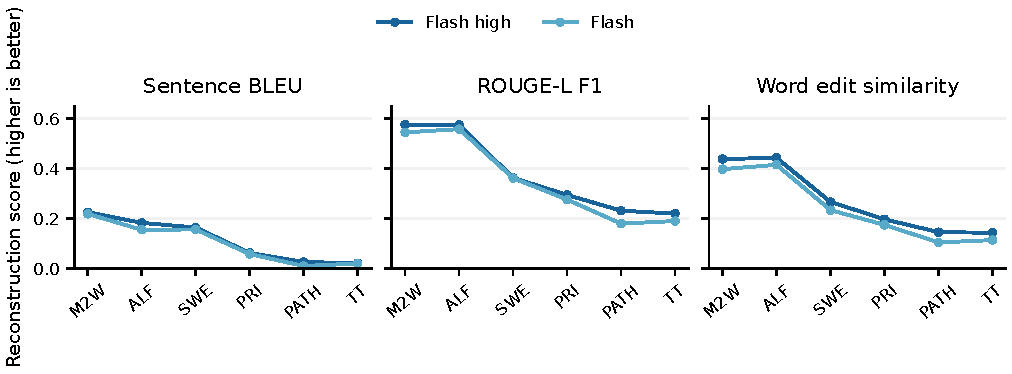
\includegraphics[width=\textwidth]{expressivity.pdf}
\caption{Mean round-trip scores by dataset for 46 reconstructions per Gemini condition (7--8 per dataset). M2W: Mind2Web; ALF: ALFRED; SWE: SWE-bench; PRI: PRISM; PATH: PATHs; TT: ThoughtTrace. Higher is better. Scores reflect both encoder and decoder behavior and include a small number of failed encodings.}
\label{fig:expressivity}
\end{figure*}

High-effort Flash averages 0.114 BLEU, 0.380 ROUGE-L, and 0.275 word edit similarity; Flash averages 0.103, 0.355, and 0.242, respectively. The small differences are descriptive, without a significance claim. Figure~\ref{fig:expressivity} shows better reconstruction for constrained instructions than open-ended dialogue. The accompanying qualitative report identifies compression, paraphrase, merged or split steps, and losses of numbers, names, or qualifications. For example, one Flash ALFRED reconstruction drops a book title retained by high-effort Flash; a PATHs height description loses a numerical value; a French ThoughtTrace conversation returns largely in English. Conversely, rewriting a third as approximately 33.33\% is not necessarily information loss. These cases explain why lexical mismatch is neither sufficient nor necessary evidence of semantic failure. Nevertheless, repeated omission of specific content limits claims that the representation preserves rich conversations.

\subsection{Reasoning improvement (RQ3)}
We use 50 items from BBEH-mini \citep{kazemi2025bbeh}, stratified over all 23 task types: two per task plus four additional sampled items (seed 2026). Llama 3.1 8B Instruct \citep{grattafiori2024llama} completes three repeats per item and condition through the Hugging Face router/DeepInfra endpoint, with temperature 0.6, top-$p$ 0.9, and at most 4,096 output tokens. The direct baseline receives the original task and a step-by-step instruction with the benchmark answer prefix. The treatment first translates with the specification and retrieved glossary, then solves in a fresh context from the translation plus language context. It does not retain the original task in the solving prompt.

\begin{table}[t]
\centering\small
\setlength{\tabcolsep}{5pt}
\begin{tabular}{lrrr}
\toprule
Task & $n$ & Direct & \bc{}\\\midrule
Boardgame QA & 6 & 1 (16.7) & 0 (0.0) \\
Boolean Expressions & 6 & 0 (0.0) & 0 (0.0) \\
Buggy Tables & 6 & 0 (0.0) & 0 (0.0) \\
Causal Understanding & 6 & 1 (16.7) & 0 (0.0) \\
Disambiguation QA & 6 & 5 (83.3) & 1 (16.7) \\
Dyck Languages & 6 & 0 (0.0) & 0 (0.0) \\
Geometric Shapes & 6 & 0 (0.0) & 0 (0.0) \\
Hyperbaton & 6 & 0 (0.0) & 0 (0.0) \\
Linguini & 6 & 0 (0.0) & 0 (0.0) \\
Movie Recommendation & 6 & 1 (16.7) & 0 (0.0) \\
Multistep Arithmetic & 6 & 0 (0.0) & 0 (0.0) \\
NYCC & 6 & 2 (33.3) & 0 (0.0) \\
Object Counting & 6 & 0 (0.0) & 0 (0.0) \\
Object Properties & 6 & 0 (0.0) & 0 (0.0) \\
SARC Triples & 6 & 3 (50.0) & 0 (0.0) \\
Shuffled Objects & 9 & 2 (22.2) & 0 (0.0) \\
Spatial Reasoning & 6 & 0 (0.0) & 0 (0.0) \\
SportQA & 9 & 0 (0.0) & 0 (0.0) \\
Temporal Sequence & 9 & 0 (0.0) & 0 (0.0) \\
Time Arithmetic & 6 & 1 (16.7) & 0 (0.0) \\
Web Of Lies & 6 & 0 (0.0) & 0 (0.0) \\
Word Sorting & 9 & 1 (11.1) & 0 (0.0) \\
Zebra Puzzles & 6 & 1 (16.7) & 0 (0.0) \\
\midrule
\textbf{Total} &\textbf{150}&\textbf{18 (12.0)}&\textbf{1 (0.7)}\\
\bottomrule
\end{tabular}
\caption{BBEH-mini correct runs (accuracy in percent) by every sampled task type. $n$ is the number of runs per condition, three per item. Scores use the benchmark evaluator; no runs errored.}
\label{tab:improvement}
\end{table}

Accuracy falls from 18/150 (12.0\%) to 1/150 (0.7\%), an 11.3-point decline (Table~\ref{tab:improvement}). The item-clustered GEE check gives $p=0.0014$; a Bayesian random-intercept logistic model estimates an odds ratio of 0.05 (approximate 95\% interval 0.01--0.19). However, majority voting within each item yields only five baseline-only successes and no treatment-only successes: exact paired McNemar $p=0.0625$. The negative direction is consistent, while the strength of statistical evidence depends on aggregation and model assumptions.

Only 54\% of treatment translations contain a recognized \code{braincode} block; otherwise the implementation forwards the entire translation response. Consequently this experiment tests the practical two-stage prompting pipeline, including its translation and formatting failures, not the intrinsic usefulness of perfectly formed \bc{}. Large language context, information loss, and lack of language-specific training are plausible explanations, but were not isolated by ablations. There is no matched-compute or alternative structured-notation control. We prepared a fine-tuning attempt, but resource constraints prevented an evaluated trained model; it cannot support a claim that training would reverse the result.

\section{Conclusions and Discussion}
\subsection{Conclusions}
\paragraph{Agent-created language (RQ2).}
Agents and human reviewers produced a substantial specification and glossary designed for readability; several models accepted most held-out translations. Yet noun grouping remained a recurring development and evaluation bottleneck: open object labels must support new values without silently inventing semantics, while closed definitions demand continuing enumeration. Failure reports identify this as a central problem without quantifying its causal share. High acceptance also coexists with lossy reconstructions, so coverage alone is insufficient evidence of a well-functioning language.

Haiku exceeds Sonnet despite their expected capability ordering; Gemini exceeds Sonnet and the OpenAI conditions, but not Haiku. This suggests adaptation to the Gemini-led swarm, or a division between lenient readers (Gemini and Haiku) and stricter readers demanding dedicated constructions. Mixing formal constraints with prose meanings leaves difficult interpretive ambiguities that our process did not resolve across model families.

\paragraph{Comparative research (RQ1).}
Symbol distributions reveal decomposition and vocabulary preferences, making \bc{} a promising behavioral probe. It is not a ready-to-use comparative method: construction-model bias, failures, and checker strictness can confound linguistic tendencies. Repeated construction and independent semantic judgments must establish whether these preferences are robust.

\paragraph{Reasoning (RQ3).}
In-context use harmed performance in the tested setting. Neither a decomposition benefit nor context length as the cause is established. Fine-tuning could reduce the need to supply documentation and improve language fluency, but our unfinished attempt leaves that hypothesis open. Further assessment must separate representation, translation, and prompting costs.

\subsection{Limitations}
Our six sources cover limited natural-language domains, with only 18 shared evaluation items and one reasoning model tested on 50 items. Repeats do not create independent tasks. We do not isolate effects of loop design, retrieval, consolidation, or human intervention.

Proxy request limits constrained swarm development and required interventions, including prompt adaptations and changes to command access during runs. Their indirect effects remain unmeasured: a frozen evaluation snapshot does not make development a controlled ablation. Model labels and proxy endpoints also limit reproducibility of hosted-model behavior.

Except for downstream BBEH scoring, our evaluations are tailored to this language and are exploratory rather than standardized benchmarks. The acceptance gate is incomplete, reconstruction metrics are lexical, and interpretability lacks a human study. Runtime and token efficiency were excluded as objectives; the additional translation call and documentation suggest overhead, but we did not establish an efficiency benefit. Finally, bias toward construction models limits the fairness of using \bc{} to compare other models.

\subsection{Future work}
With more resources, we would automate syntax and glossary maintenance while explicitly evaluating which human checks can be removed. Few-shot examples and more selective retrieval could improve compatibility and reduce time and context costs. A glossary swarm spanning model companies would test construction-model bias; our non-Gemini experiments were constrained by personal funding. Fine-tuning on verified translations should be compared with in-context use under held-out items and matched budgets, rather than assumed to help.

Independent creation runs could quantify structural and behavioral variance, testing whether model preferences recur across languages and strengthening both agent-capability and comparative-research conclusions. A further direction is explicit swarm communication: emergent communication research studies how agents acquire shared symbolic conventions \citep{havrylov2017language,lazaridou2020communication}. The reported Hugging Face incident illustrates the importance of observing and governing agent coordination \citep{openai2026incident}. Auditable protocols warrant study; prevention of such incidents by \bc{} is untested.

\label{maintext:end}
\clearpage
\section*{AI Disclosure}
According to the authors' development record, OpenAI Astra 6 (medium reasoning) and, predominantly, Claude Opus 5.5 assisted with code implementation from human instructions, pipeline design and refinements, adaptations to Guy's swarm infrastructure, evaluation implementation, run monitoring, improvement suggestions, dataset retrieval, and design consultation. OpenAI Astra 6 (medium reasoning) also assisted with the initial specification and glossary refinements, comparison against Guy's predefined syntax, and migration of its ideas into the syntax-loop output. Separate model agents used in the experiments are described in the main text.

An AI writing assistant prepared this manuscript from the authors' outline, inspected repository code and saved results, summarized the supplied design documents and qualitative reports, checked bibliographic sources, and generated figures from saved aggregate data. It also assisted with language editing and LaTeX layout. The reported experiments were not rerun for manuscript preparation. This disclosure describes assistance; it does not constitute an independent human validation of every semantic interpretation or generated translation.

\bibliography{references}

\clearpage
\onecolumn
\appendix
\section{Repository and Reproducibility}
\label{sec:repro}
The project repository is \url{https://github.com/liasoffer/BrainCode}. The manuscript uses the local snapshot inspected on October 6, 2026. The specification and glossary under \path{evaluations/runs/main/reference/} were compared with the current reference and found byte-identical. Core implementation and evidence locations are listed below; no claim is made that every local experimental artifact is already published remotely.

\begin{table}[H]
\centering\small
\begin{tabular}{>{\raggedright\arraybackslash}p{.25\textwidth}>{\raggedright\arraybackslash}p{.68\textwidth}}
\toprule
Purpose & Repository-relative location\\\midrule
Syntax roles and control flow & \path{syntax-loop/config/config.yaml}; \path{syntax-loop/braincode_loop/orchestrator.py}\\
Semantic migration & \path{docs/language-spec-revised.md}\\
Swarm loop and acceptance & \path{swarm/loop.py}; \path{swarm/migrate.py}; \path{swarm/inspector.py}\\
Language snapshot & \path{swarm/reference/reference-manifest.json}; specification and glossary in the same directory\\
Dataset splits & \path{swarm/data/README.md}\\
Evaluation design in code & \path{evaluations/sample.py}; \path{evaluations/run_eval.py}; \path{evaluations/metrics.py}; \path{evaluations/analyze.py}\\
Coverage, JS and reconstruction & \path{evaluations/results/main-cov-det/summary.json} and accompanying CSVs\\
Qualitative evidence & \path{evaluations/results/main-cov-det/qualitative_determinism_js.md}; \path{qualitative_expressivity_bleu_rouge_levenshtein.md} in the same directory\\
Reasoning pipeline and results & \path{evaluations/improvement/improve.py}; \path{evaluations/improvement/results/improvement_runs.csv}\\
Prepared fine-tuning data & \path{finetune-llama/data/manifest.json}\\
Manuscript and figure regeneration & \path{paper/overleaf/}; \path{paper/build_figures.py}\\
\bottomrule
\end{tabular}
\caption{Evidence map. The companion outline audit maps all requested content to manuscript locations and records changes from preliminary numbers.}
\end{table}

\paragraph{Models.}
The saved translation configuration identifies \path{vertex-proxy/gemini-flash} and \path{vertex-proxy/gemini-flash-high}, displayed as Gemini 3.7 Flash and its high-effort condition; \path{anthropic/claude-sonnet-5-5}; and \path{anthropic/claude-haiku-4-5-20251001}. Additional diagnostics use GPT-6.1 Sol, GPT-6 Luna, and o4-mini under the recorded harness configuration. These are experiment-time identifiers, not independently audited descriptions of proxy backends. The reasoning condition uses \path{meta-llama/Llama-3.1-8B-Instruct} through DeepInfra.

\begin{table}[H]
\centering\small
\begin{tabular}{lrrr}
\toprule
Dataset & Total & Local train & Local test\\\midrule
Mind2Web &2,022&1,617&405\\
ALFRED &10,001&7,975&2,026\\
SWE-bench &10,000&8,000&2,000\\
PRISM &8,011&6,408&1,603\\
PATHs &9,991&7,992&1,999\\
ThoughtTrace &2,155&1,725&430\\\midrule
Total &42,180&33,717&8,463\\
\bottomrule
\end{tabular}
\caption{Local ingestion and split counts. Each dataset contributes eight sampled evaluation items and three shared items; these counts do not describe official upstream benchmark splits.}
\end{table}

\paragraph{Prepared training and statistical scope.}
The fine-tuning manifest contains 566 examples from 279 distinct items (535 training and 31 validation examples, with disjoint item identities), assembled from 232 swarm and 334 evaluation examples. Consequently any subsequent evaluation of a model trained on these data must use a fresh language-evaluation set. No evaluated fine-tuned checkpoint is reported here. For the reasoning comparison, the saved run-level Wilson intervals are 7.7--18.2\% (direct) and 0.1--3.7\% (\bc{}), but these descriptive intervals do not account for item clustering; the paired and clustered analyses in the main text are more relevant to inference.

\section{Additional Determinism Views}
\begin{figure}[H]
\centering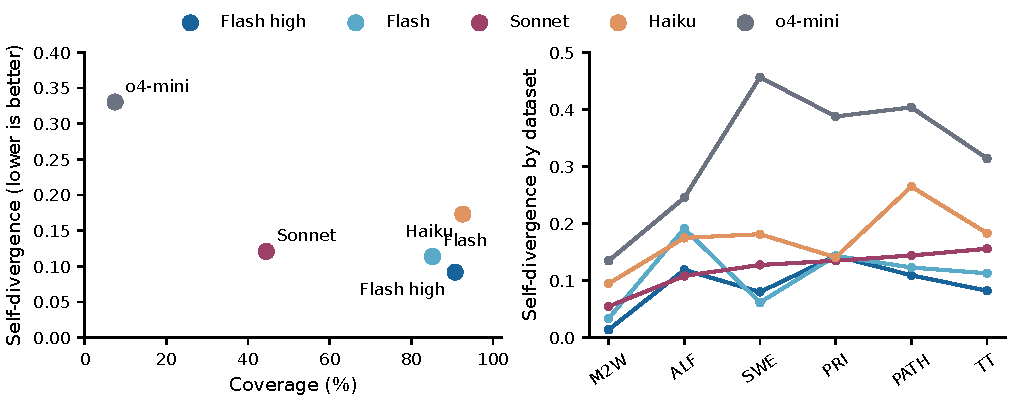
\includegraphics[width=.95\textwidth]{appendix-determinism.pdf}
\caption{Shared-set coverage versus self-divergence (left) and self-divergence by dataset (right). o4-mini is a failure-confounded diagnostic. Dataset means use only items with at least two non-error translations; there are at most three items per dataset. Abbreviations follow Figure~\ref{fig:expressivity}.}
\label{fig:appendixdet}
\end{figure}
Figure~\ref{fig:appendixdet} separates two objectives that a single success score obscures. Coverage ranks Haiku (92.6\%), high-effort Flash (90.7\%), Flash (85.2\%), Sonnet (44.4\%), and o4-mini (7.4\%). Repeat stability, from lowest to highest divergence, ranks high-effort Flash (0.092), Flash (0.114), Sonnet (0.121), Haiku (0.173), and o4-mini (0.330). Per-dataset variation is substantial: Haiku's largest divergence occurs on PATHs, while o4-mini's largest occurs on SWE-bench. These small, selected subsets support descriptive comparisons only.

\section{Page Allocation}
Estimated occupied space is 0.5 page for the abstract and title, 0.8 for the introduction, 2.3 for \bc{}, 3.4 for evaluation, and 1.0 for conclusions, limitations, and future work: eight pages in total. These estimates include floats and shared pages, rather than counting every page touched by a section. Figures and tables count toward their sections. AI disclosure, references, and appendices begin after an explicit page break and are excluded from that count. The companion page-budget document reports the final compiled allocation.
\end{document}
